% https://tex.stackexchange.com/questions/1423/is-there-a-nice-way-to-compile-a-beamer-presentation-without-the-pauses
\documentclass[handout]{beamer}
%\documentclass[]{beamer}
% http://tex.stackexchange.com/questions/34265/how-to-get-beamer-math-to-look-like-article-math
% https://tex.stackexchange.com/questions/54905/how-to-modify-default-beamercolortheme
\usefonttheme[onlymath]{serif}
\include{graphix}
\include{amsmath}
% http://tex.stackexchange.com/questions/14688/put-variable-text-at-a-fixed-location-on-every-beamer-slide
\usepackage[absolute,overlay]{textpos}  
\usepackage{hyperref}
% http://tex.stackexchange.com/questions/99359/putting-animations-into-latex-beamer-presentation-use-png-gif
\usepackage{animate}
\usepackage{tikz}
% https://tex.stackexchange.com/questions/86500/includegraphics-set-image-opacity
\usepackage{transparent}
\usepackage{pgf}
% https://tex.stackexchange.com/questions/40666/how-to-change-line-color-in-tabular
\usepackage{colortbl} 
% https://en.wikibooks.org/wiki/LaTeX/Tables
\usepackage{multirow}  % Columns spanning multiple rows
% http://tex.stackexchange.com/questions/122880/continuing-example-counters-in-beamer
\setbeamertemplate{theorem}[ams style]
\setbeamertemplate{theorems}[numbered]
\newenvironment{example*}
  {\addtocounter{theorem}{-1}\example}
  {\endexample}
  
%http://tex.stackexchange.com/questions/73718/frame-numbering-in-warsaw-theme
\expandafter\def\expandafter\insertshorttitle\expandafter{%
    \insertshorttitle\hfill\insertframenumber\,/\,\inserttotalframenumber}
\expandafter\def\expandafter\insertauthor\expandafter{%
    \insertauthor\hfill\text{rev 12}}

% http://tex.stackexchange.com/questions/112598/beamer-grey-out-items-after-pause
\setbeamercovered{transparent}

\newcommand{\pathname}[0] {../common/}
\newcommand{\fullpath}[0] {\pathname}
\newcommand{\clr}[0]      {violet}

\input{\pathname declarations.tex}
\input{\pathname packages.tex}
%\setbeamercolor{author in head/foot}{bg=White}

\title{Fixing Gauge and Rank Deficiency}
%\author[Topa, Embid]{\authorTopa \\ \authorEmbid }% \\ \authorTopa}
% \fontsize{20}{25}\selectfont
\author[\mg{\fontsize{5}{15}\selectfont DISTRIBUTION A. Approved for public release: distribution unlimited.}]{}
%\date{29 July 2015}
\begin{document}

% http://tex.stackexchange.com/questions/237396/logo-top-right-latex-beamer-warsaw-presentation
\addtobeamertemplate{headline}{}{%
\begin{tikzpicture}[remember picture,overlay]
\node at([shift={(0.42\paperwidth,-0.47)}]current page.north) {
\includegraphics[ height = 0.75cm ]{../graphics/logos/HPCMP}};
\end{tikzpicture}}

\tpage

%  %  %  %  %  %  %  %  %  %  %  %  %  %  %  %  %  %  %  %  %  %  %  %  %  %  %  %  %  %  %  %  %  %  %  %  %  %  %  %  %  %  %  %  %  %  %
\section{Goal}

\begin{frame}      %  %  %   FRAME   %  %  %
\frametitle{Equivalent Statements}
  %
  Fix gauge to fix rank deficiency \\[20pt]
  \pause
  %
  Input $\aicmnr$, construct $\aicmrr$  \\[20pt]
  \pause
  %
  Given $\A{} = \csvdblockb{*}$, dim$\paren{\rvn{}} \to 0$
  %
  %
  %
\end{frame}


%  %  %  %  %  %  %  %  %  %  %  %  %  %  %  %  %  %  %  %  %  %  %  %  %  %  %  %  %  %  %  %  %  %  %  %  %  %  %  %  %  %  %  %  %  %  %
\section{Background}

%  %%  %%  %%  %%  %%  %%  %%  %%  %%  %%  %%  %%  %%  %%  %%  %%  %%  %%  %%  %%  %%  %%  %%  %%  %%  %%  %%  %%  %%  %%  %%  %%  %%  %%
\subsection{Gauge Basics}

\begin{frame}      %  %  %   FRAME   %  %  %
\frametitle{Central Questions}
  %
  What does a gauge function measure?  Displacement in superfluous degrees of freedom.\\[20pt]
  %
  \pause
  %
  Why fix the gauge? To handle redundant degrees of freedom and simplify computation.
  %
\end{frame}

\begin{frame}
  \frametitle{Redundant Degrees of Freedom: $\axeb$}  % - - - - F R A M E
  %
  \begin{center}
    \includegraphics[ width = 3in ]{../graphics/strays/"least squares wide domain"}
  \end{center}
  %
\end{frame}


\begin{frame}      %  %  %   FRAME   %  %  %
\frametitle{Electrodynamics: Example}
  %
  Maxwell's equations \\
  %
\begin{table}[htdp]
  %\caption{default}
  \begin{center}
    \begin{tabular}{ll}
      %
      divergence & curl \\\hline
      %
      \\
      %
      $\nabla \cdot \D{} = 4 \pi \rho$ &
      $\nabla \times \E{} = - \frac{1}{c} \pdt{\B{}}$ \\[10pt]
      %
      $\nabla \cdot \B{} = 0$ &
      $\nabla \times \HH{} = \frac{4\pi}{c} \J{} + \frac{1}{c} \pdt{\D{}}$
      %
    \end{tabular}
  \end{center}
  %\label{default}
\end{table}%
  %
\end{frame}

\begin{frame}
  \frametitle{Electrodynamics: Vector and Scalar Potentials}  % - - - - F R A M E
  %
  $$\B{} = \nabla \times \A{}$$\\[20pt]
  %
  $$\E{} = - \nabla \phi - \frac{1}{c} \pdt{\A{}}$$
  %
\end{frame}

\begin{frame}      %  %  %   FRAME   %  %  %
\frametitle{Electrodynamics: Gauge Fixing Conditions}
  %
  \begin{center}
  Coulomb:
  \end{center}
  $$ \nabla \cdot \A{}\paren{\mathbf{r}, t} \bl{ = 0}$$ \\[20pt]
  %
  \begin{center}
  Lorenz:
  \end{center}
  $$ \partial^{\mu} A_{\mu} \bl{ = 0}$$ \\
  \begin{center}
     or...
  \end{center}
  $$ \nabla \cdot {\A{}}({\bf{r}}, t) + \frac{1}{c^{2}} \frac{\partial \phi}{\partial t} \bl{= 0}$$
  %
\end{frame}

%  %%  %%  %%  %%  %%  %%  %%  %%  %%  %%  %%  %%  %%  %%  %%  %%  %%  %%  %%  %%  %%  %%  %%  %%  %%  %%  %%  %%  %%  %%  %%  %%  %%  %%
\subsection{Scalar Potentials}

\begin{frame}      %  %  %   FRAME   %  %  %
\frametitle{Scalar Potentials $\phi$}
  %
  Sobolev Space:
  %
$$W^{1,2}\left( \Omega \right) = \left\{ \phi\in L^{2}\left( \Omega \right)\colon \partial_{x}^{1}\phi\in L^{2}\left( \Omega \right) \right\}$$
  %
\end{frame}

%  %%  %%  %%  %%  %%  %%  %%  %%  %%  %%  %%  %%  %%  %%  %%  %%  %%  %%  %%  %%  %%  %%  %%  %%  %%  %%  %%  %%  %%  %%  %%  %%  %%  %%
\subsection{Gradients}

\begin{frame}      %  %  %   FRAME   %  %  %
\frametitle{Prototype Vector Field Equation}
  %
  $$\bf{E} = - \nabla \phi$$ \\[20pt]
  \onedot
  %
  \pause
  %
  \begin{center}
    Inverse problem: Measure $\bf{E}$ find $\phi$
  \end{center}
  \onedot
  %
\end{frame}

%  %%  %%  %%  %%  %%  %%  %%  %%  %%  %%  %%  %%  %%  %%  %%  %%  %%  %%  %%  %%  %%  %%  %%  %%  %%  %%  %%  %%  %%  %%  %%  %%  %%  %%
\subsection{Least Squares}

\begin{frame}      %  %  %   FRAME   %  %  %
\frametitle{Least Squares: Problem}
  %
  $$\axeb$$\\[0pt]
  %%
  \begin{itemize}
		\item system matrix $\A{}\colon \cmplxn \mapsto \cmplxm$
		\item data vector $b \in \cmplxm$
	\end{itemize}
	%%
	Least squares solution
	$$x_{LS} = \lst{ x\in\cmplxn{} \colon \minimum{} \text{ is minimized} }$$
  %
\end{frame}

\begin{frame}      %  %  %   FRAME   %  %  %
\frametitle{Least Squares: Solution}
  %
  $$\axeb$$ \\[10pt]
  %
  \pause
  %
  $$x_{LS} = \solnls{b}{y}, \qquad y\in\cmplxn$$ \\[10pt]
  %
  \begin{center}
     or...
  \end{center}
  %
  $$x_{LS} = \Ap b + \pras y, \qquad y\in\cmplxn$$ \\[10pt]
  %
\end{frame}

\begin{frame}      %  %  %   FRAME   %  %  %
\frametitle{Least Squares: Invariance}
  %
  $$x_{*} = \Ap b$$ \\[10pt]
  %
  $$x_{*} \rightarrow x_{*} + \pras y$$ \\[10pt]
  %
  $$\A{}\paren{x_{*}} = \A{}\paren{x_{*} + \pras y}$$
  %
  \twodots
  %
\end{frame}

%  %  %  %  %  %  %  %  %  %  %  %  %  %  %  %  %  %  %  %  %  %  %  %  %  %  %  %  %  %  %  %  %  %  %  %  %  %  %  %  %  %  %  %  %  %  %
\section{Least Squares - Modal}

%  %%  %%  %%  %%  %%  %%  %%  %%  %%  %%  %%  %%  %%  %%  %%  %%  %%  %%  %%  %%  %%  %%  %%  %%  %%  %%  %%  %%  %%  %%  %%  %%  %%  %%
\subsection{Approximation}

\begin{frame}      %  %  %   FRAME   %  %  %
\frametitle{Approximating Measurement}
  %
  \begin{enumerate}
    \item Select \bl{modes}: basis functions $\lst{g_{\nu}(x)}_{\nu=1}^{n}$ \\[15pt]
    \item Find amplitudes $a$ to describe measured function $f(x)$ \\[15pt]
  \end{enumerate}
  %
  %
  $$f ( x ) \approx a_{1} g_{1}(x) + a_{2} g_{2}(x) + a_{3} g_{3}(x) + \dots = \sum\limits_{\nu=1}^{n} a_{\nu} g_{\nu}(x)$$ 
  %
\end{frame}

\begin{frame}      %  %  %   FRAME   %  %  %
\frametitle{Merit Function}
  %
  $$M(a) = \sum_{k = 1}^{m} r_{k}^{2}$$
  %
  \pause
  %
  $$r_{k} = f(x_{k}) - \sum_{\nu = 1}^{n} a_{\nu} g_{\nu}(x_{k})$$
  %
  \pause
  %
  $$M(a) = \sum_{k = 1}^{m} \paren{f(x_{k}) - \sum_{\nu = 1}^{n} a_{\nu} g_{\nu}(x_{k})}^{2}$$
  %
  %
\end{frame}

\begin{frame}      %  %  %   FRAME   %  %  %
\frametitle{Example: Vectors}
  %
  $$g(x) = \lst{ 1, x, x^{2}, x^{3} }$$\\[20pt]
  %
  $${\bf{1}} = \mat{c}{1\\[4pt]1\\\vdots\\[4pt]1}, \quad
          {\bf{x}} =\mat{c}{x_{1}\\[4pt]x_{2}\\\vdots\\[4pt]x_{m}}, \quad
          {\bf{x}}^{2} =\mat{c}{x_{1}^{2}\\[4pt]x_{2}^{2}\\\vdots\\[4pt]x_{m}^{2}}, \quad
          {\bf{x}}^{3} =\mat{c}{x_{1}^{3}\\[4pt]x_{2}^{3}\\\vdots\\[4pt]x_{m}^{3}}$$
  %
\end{frame}


%  %%  %%  %%  %%  %%  %%  %%  %%  %%  %%  %%  %%  %%  %%  %%  %%  %%  %%  %%  %%  %%  %%  %%  %%  %%  %%  %%  %%  %%  %%  %%  %%  %%  %%
\subsection{Gauge Fixing}

\begin{frame}      %  %  %   FRAME   %  %  %
\frametitle{Gauge Fixing Conditions}
  %
  \begin{table}[htdp]
    %\caption{default}
    \begin{center}
      \begin{tabular}{lll}
        %
        $\partial_{1}M$ & ${\bf{r}} \cdot {\bf{1}} = 0$     & $\sum\limits_{k = 1}^{m} r_{k} = 0$ \\[15pt]
        %
        $\partial_{2}M$ & ${\bf{r}} \cdot {\bf{x}} = 0$     & $\sum\limits_{k = 1}^{m} r_{k}x_{k} = 0$ \\[15pt]
        %
        $\partial_{3}M$ & ${\bf{r}} \cdot {\bf{x}}^{2} = 0$ & $\sum\limits_{k = 1}^{m} r_{k}x_{k}^{2} = 0$ \\[15pt]
        %
        $\partial_{4}M$ & ${\bf{r}} \cdot {\bf{x}}^{3} = 0$ & $\sum\limits_{k = 1}^{m} r_{k}x_{k}^{3} = 0$ \\[15pt]
        %
      \end{tabular}
    \end{center}
    %\label{default}
  \end{table}%
  \onedot
  %
\end{frame}


\begin{frame}      %  %  %   FRAME   %  %  %
\frametitle{Gauge Fixing Conditions}
  %
  \begin{table}[htdp]
    %\caption{default}
    \begin{center}
      \begin{tabular}{lll}
        %
        $\bl{\partial_{1}M}$ & $\bl{{\bf{r}} \cdot {\bf{1}} = 0}$     & $\bl{\sum\limits_{k = 1}^{m} r_{k} = 0}$ \\[15pt]
        %
        $\partial_{2}M$ & ${\bf{r}} \cdot {\bf{x}} = 0$     & $\sum\limits_{k = 1}^{m} r_{k}x_{k} = 0$ \\[15pt]
        %
        $\partial_{3}M$ & ${\bf{r}} \cdot {\bf{x}}^{2} = 0$ & $\sum\limits_{k = 1}^{m} r_{k}x_{k}^{2} = 0$ \\[15pt]
        %
        $\partial_{4}M$ & ${\bf{r}} \cdot {\bf{x}}^{3} = 0$ & $\sum\limits_{k = 1}^{m} r_{k}x_{k}^{3} = 0$ \\[15pt]
        %
      \end{tabular}
    \end{center}
    %\label{default}
  \end{table}%
  \twodots
  %
\end{frame}

\begin{frame}      %  %  %   FRAME   %  %  %
\frametitle{Summary}
  %
    \begin{center}
      \Huge{Forming the normal equations =\\
      imposing a gauge condition}
    \end{center}
  \twodots
  %
\end{frame}

%  %  %  %  %  %  %  %  %  %  %  %  %  %  %  %  %  %  %  %  %  %  %  %  %  %  %  %  %  %  %  %  %  %  %  %  %  %  %  %  %  %  %  %  %  %  %
\section{Least Squares - Zonal}

\begin{frame}      %  %  %   FRAME   %  %  %
\frametitle{Measurement of Average Gradient}
	%
	Partition a domain: \\
	$$\Omega = \bigcup_{k} \omega_{k}$$ \\
  %
  Interval \\
  $$\omega = \lst{x \in\real{} \colon \bl{a} < x < \bl{b}}$$ \\
  \pause
  %
  Average gradient \\
  $$\langle \nabla \phi(x) \rangle_{\omega} = \phi(\bl{b}) - \phi(\bl{a})$$
  %
  \onedot
  %
\end{frame}

\begin{frame}      %  %  %   FRAME   %  %  %
\frametitle{Measurement of Average Gradient}
	%
	\mg{
	Partition a domain: \\
	$$\Omega = \bigcup_{k} \omega_{k}$$ \\
  %
  Interval \\
  $$\omega = \lst{x \in\real{} \colon a < x < b}$$} \\
  %
  Average gradient \\
  $$\boxed{\langle \nabla \phi(x) \rangle_{\omega} = \phi(\bl{b}) - \phi(\bl{a})}$$
  %
\end{frame}

%  %%  %%  %%  %%  %%  %%  %%  %%  %%  %%  %%  %%  %%  %%  %%  %%  %%  %%  %%  %%  %%  %%  %%  %%  %%  %%  %%  %%  %%  %%  %%  %%  %%  %%
\subsection{1 Dimension}

\begin{frame}      %  %  %   FRAME   %  %  %
\frametitle{Source of Rank Defect}
  %
  $$D_{x} \phi(x) = D_{x} \paren{\phi(x) + const}$$
  %
\end{frame}

\begin{frame}      %  %  %   FRAME   %  %  %
\frametitle{Scalar Potential $\phi$}
  %
  \begin{center}
    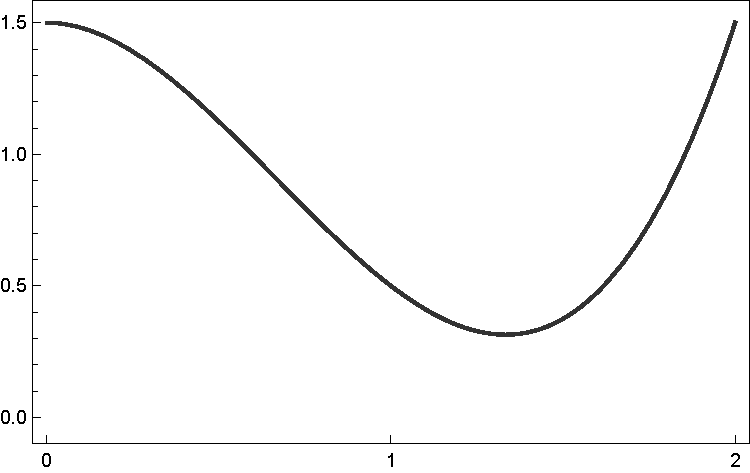
\includegraphics[ width = 3.5in ]{../graphics/"one d"/phi}
  \end{center}
  %
\end{frame}

\begin{frame}      %  %  %   FRAME   %  %  %
\frametitle{Scalar Potential $\phi$: Zone 1}
  %
  \begin{center}
    \includegraphics[ width = 3.5in ]{../graphics/"one d"/"device left"}
  \end{center}
  %
  \begin{textblock}{2.75}(4.35,7.25)
    $\bl{\omega_{1}}$
  \end{textblock}
  %
\end{frame}

\begin{frame}      %  %  %   FRAME   %  %  %
\frametitle{Scalar Potential $\phi$: Zone 2}
  %
  \begin{center}
    \includegraphics[ width = 3.5in ]{../graphics/"one d"/"device right"}
  \end{center}
  %
  \begin{textblock}{2.75}(8.5,7.25)
    $\bl{\omega_{2}}$
  \end{textblock}
  %
\end{frame}

\begin{frame}      %  %  %   FRAME   %  %  %
\frametitle{Scalar Potential $\phi$: Endpoints}
  %
  \begin{center}
    \includegraphics[ width = 3.5in ]{../graphics/"one d"/"connect dots"}
  \end{center}
  %
\end{frame}

\begin{frame}      %  %  %   FRAME   %  %  %
\frametitle{Scalar Potential $\phi$: Average Gradient}
  %
  \begin{center}
    \includegraphics[ width = 3.5in ]{../graphics/"one d"/"average gradient"}
  \end{center}
  %
\end{frame}

\begin{frame}      %  %  %   FRAME   %  %  %
\frametitle{Scalar Potential $\phi$: Measurement and Solution}
  %
  \begin{center}
    \includegraphics[ width = 3.5in ]{../graphics/"one d"/"sticks 02"}
  \end{center}
  %
\end{frame}

\begin{frame}      %  %  %   FRAME   %  %  %
\frametitle{Scalar Potential $\phi$: Input and Output}
  %
  \begin{center}
    \includegraphics[ width = 3.5in ]{../graphics/"one d"/"sticks 04"}
  \end{center}
  %
\end{frame}

\begin{frame}      %  %  %   FRAME   %  %  %
\frametitle{Scalar Potential $\phi$: Least Squares Solution}
  %
  \begin{center}
    \includegraphics[ width = 3.5in ]{../graphics/"one d"/"sticks 05"}
  \end{center}
  %
\end{frame}

\begin{frame}      %  %  %   FRAME   %  %  %
\frametitle{Scalar Potential $\phi$: Rosetta Stone}
  %
  \begin{center}
    \includegraphics[ width = 3.5in ]{../graphics/"one d"/"sticks dots"}
  \end{center}
  \begin{textblock}{2.75}(4.45,4.25)
    $\bl{x_{1}}$
  \end{textblock}
  %
  \begin{textblock}{2.75}(8.25,4.25)
    $\bl{x_{2}}$
  \end{textblock}
  %
  \begin{textblock}{2.75}(2.85,2.90)
    $\varphi_{0}$
  \end{textblock}
  %
  \begin{textblock}{2.75}(6.35,5.80)
    $\varphi_{1}$
  \end{textblock}
  %
  \begin{textblock}{2.75}(9.95,2.9)
    $\varphi_{2}$
  \end{textblock}
  %
\end{frame}

\begin{frame}      %  %  %   FRAME   %  %  %
\frametitle{Scalar Potential $\phi$: Rosetta Stone}
  %
  \begin{center}
    \includegraphics[ width = 3.5in ]{../graphics/"one d"/"sticks dots"}
  \end{center}
  \begin{textblock}{2.75}(4.45,4.25)
    $\bl{x_{1}}$
  \end{textblock}
  %
  \begin{textblock}{2.75}(8.25,4.25)
    $\bl{x_{2}}$
  \end{textblock}
  %
  \begin{textblock}{2.75}(2.85,2.90)
    $\varphi_{0}$
  \end{textblock}
  %
  \begin{textblock}{2.75}(6.35,5.80)
    $\varphi_{1}$
  \end{textblock}
  %
  \begin{textblock}{2.75}(9.95,2.9)
    $\varphi_{2}$
  \end{textblock}
  %
  \begin{textblock}{2.75}(3.5,6.9)
    $\varphi_{1} - \varphi_{0} = x_{1}$
  \end{textblock}
  %
  \begin{textblock}{2.75}(7.5,6.9)
    $\varphi_{2} - \varphi_{1} = x_{2}$
  \end{textblock}
  %
\end{frame}

\begin{frame}      %  %  %   FRAME   %  %  %
\frametitle{Linear System}
  %
  Linear system
  %
  $$\mat{rrc}{-1 & 1 & 0 \\ 0 & -1 & 1}\mat{c}{\varphi_{0} \\ \varphi_{1} \\ \varphi_{2}} = \mat{c}{x_{1} \\ x_{2}}$$
  %
  \bdoton
  \pause
  Least squares solution
  %
  $$\mat{c}{\varphi_{0} \\ \varphi_{1} \\ \varphi_{2}} = \frac{1}{3} \mat{rr}{ -2 & -1 \\ 1 & -1 \\ 1 & 2 } \mat{c}{x_{1} \\ x_{2}} + \alpha \rd{\mat{c}{1\\1\\1}}$$
  %
\end{frame}

\begin{frame}      %  %  %   FRAME   %  %  %
\frametitle{Gauge Condition}
  %
    Least squares solution
  %
  $$\mat{c}{\varphi_{0} \\ \varphi_{1} \\ \varphi_{2}} = \frac{1}{3} 
  \underbrace{\mat{rr}{ -2 & -1 \\ 1 & -1 \\ 1 & 2 }}_{\text{columns sum to } 0} \mat{c}{x_{1} \\ x_{2}} + \alpha 
  				\rd{\mat{c}{1\\1\\1}}$$
  %
\end{frame}

\begin{frame}      %  %  %   FRAME   %  %  %
\frametitle{Gauge Fixing Condition}
  %
  $$ \sum_{k} \varphi_{k} = 0 $$ \\[10pt]
  %
  $$ \Downarrow $$ \\[10pt]
  %
  $$ \mat{rr}{-1 & 1 \\ -2 & -2} \mat{c}{ \varphi_{0} \\ \varphi_{1} } = \mat{c}{x_{1} \\ x_{2}} $$
  %
\end{frame}

\begin{frame}      %  %  %   FRAME   %  %  %
\frametitle{Linear System: Fixed Gauge}
  %
  \begin{table}[htdp]
    %\caption{default}
    \begin{center}
      \begin{tabular}{ccc}
        %
        $\varphi_{0} + \varphi_{1} + \varphi_{2} = 0$
          & $\Longrightarrow$ &
        $\varphi_{2} = -\varphi_{0} - \varphi_{1}$ \\[10pt]
        %
        \pause
        %
        $\varphi_{2} - \varphi_{1} = x_{2}$ 
          & $\Longrightarrow$ &
        $-\varphi_{0} - 2 \varphi_{0} = x_{2}$ \\[10pt]
        %
        \pause
        %
        $\mat{rrc}{-1 & 1 & 0 \\ 0 & -1 & 1}\mat{c}{\varphi_{0} \\ \varphi_{1} \\ \varphi_{2}}$
          & $\Longrightarrow$ &
        $\mat{rr}{-1 & 1 \\ -1 & -2} \mat{c}{ \varphi_{0} \\ \varphi_{1} }$
        %
      \end{tabular}
    \end{center}
    %\label{default}
  \end{table}  
  %
\end{frame}

\begin{frame}      %  %  %   FRAME   %  %  %
\frametitle{Compare Solutions}
  %
    \begin{table}[htdp]
        %\caption{default}
        \begin{center}
            \begin{tabular}{ll}
              %
              Least squares solution & Fixed gauge solution \\\hline
              %
              \\
              %
              $\varphi_{0} = \frac{1}{3} \paren{ -2x_{1} - x_{2} } + \alpha$ & $\varphi_{0} = \frac{1}{3} \paren{ -2x_{1} - x_{2} }$ \\[10pt]
              %
              $\varphi_{1} = \frac{1}{3} \paren{ x_{1} - x_{2} } + \alpha$ & $\varphi_{1} = \frac{1}{3} \paren{ x_{1} - x_{2} }$ \\[10pt]
              %
              $\varphi_{2} = \frac{1}{3} \paren{ x_{1} + 2 x_{2} } + \alpha$
              %
            \end{tabular}
        \end{center}
        %\label{default}
    \end{table}%
  %
  \pause
  %
  \ \\[10pt]
  From gauge condition:
  %
  $$\varphi_{2} = -\varphi_{1} -\varphi_{0} = \frac{1}{3} \paren{ x_{1} + 2 x_{2} }$$ \\
  %
  \twodots
  %
\end{frame}

%  %%  %%  %%  %%  %%  %%  %%  %%  %%  %%  %%  %%  %%  %%  %%  %%  %%  %%  %%  %%  %%  %%  %%  %%  %%  %%  %%  %%  %%  %%  %%  %%  %%  %%
\subsection{Unit Cells}

\begin{frame}      %  %  %   FRAME   %  %  %
\frametitle{Unit Cells}
  %
  \begin{table}[htdp]
    \begin{center}
      \begin{tabular}{cccc}
        %
        \includegraphics[ width = 1.2in ]{../graphics/units/"unit 2"} &
        %
        \includegraphics[ width = 1.2in ]{../graphics/units/"unit 3"} &
        %
        \includegraphics[ width = 1.2in ]{../graphics/units/"unit 4"} \\
        %
        $d = 2$ &
        %
        $d = 3$ &
        %
        $d = 4$
        %
      \end{tabular}
    \end{center}
    %\label{default}
    %\caption{default}
  \end{table}%
  %
\end{frame}

\begin{frame}
\frametitle{Source of Rank Defects} %  %  %   FRAME   %  %  %
  %
  \begin{table}[htdp]  %  T A B L E
    %\caption{default}
    \begin{center}
      \begin{tabular}{cc}
      	%
		rank defect & invariance \\\hline
		%
		\ \\
        %
        1 & $D_{x}\phi(x) = D_{x}\paren{\phi(x) + c}$ \\[15pt]
        %
        \multirow{2}*{\bl{2}}
          & $\partial_{x}\phi(x,y) = \partial_{x}\paren{\phi(x,y) + \bl{c_{1}}}$ \\[10pt]
          & $\partial_{y}\phi(x,y) = \partial_{y}\paren{\phi(x,y) + \bl{c_{2}}}$ \\[15pt]
        %
        \multirow{3}*{\pr{3}}
          & $\partial_{x}\phi(x,y,z) = \partial_{x}\paren{\phi(x,y,z) + \pr{c_{1}}}$ \\[10pt]
          & $\partial_{y}\phi(x,y,z) = \partial_{y}\paren{\phi(x,y,z) + \pr{c_{2}}}$ \\[10pt]
          & $\partial_{z}\phi(x,y,z) = \partial_{z}\paren{\phi(x,y,z) + \pr{c_{3}}}$ \\[15pt]
        %
      \end{tabular}
    \end{center}
  %\label{default}
  \end{table}%
  %
  \twodots
  %
\end{frame}

%  %%  %%  %%  %%  %%  %%  %%  %%  %%  %%  %%  %%  %%  %%  %%  %%  %%  %%  %%  %%  %%  %%  %%  %%  %%  %%  %%  %%  %%  %%  %%  %%  %%  %%
\subsection{Dimensions 2 and 3}

\begin{frame}
  \frametitle{Average Gradient}  % - - - - F R A M E
  %
  Motivates geometric interpretation of null space vectors
  %
\end{frame}

\begin{frame}
  \frametitle{Average Gradient: Unit Cell}  % - - - - F R A M E
  %
  \begin{center}
    \includegraphics[ width = 2.00 in ]{../graphics/rectangles/"rect vec"}
  \end{center}
  %
\end{frame}

\begin{frame}
  \frametitle{Average Gradient: Unit Cell}  % - - - - F R A M E
  %
  \begin{center}
    \includegraphics[ width = 2.00 in ]{../graphics/rectangles/"rect signs phi"}
  \end{center}
  %
\end{frame}

\begin{frame}
  \frametitle{Antiderivative}  % - - - - F R A M E
  %
  $$\Phi_{\mu}(x_{1}, x_{2}) = \int \phitwo dx_{\mu}$$
  %
\end{frame}

\begin{frame}
  \frametitle{Average Gradient}  % - - - - F R A M E
  %  e q u a t i o n
\begin{equation*}
  \begin{split}
    \langle \partial_{\mu} \phitwo \rangle_{p} 
      &= \int \int \partial_{\mu} \phitwo dx_{\mu} dx_{\nu} \\
      &= \Phi_{\nu}(p) + \Phi_{\nu}(p + \hat{x}_{1} + \hat{x}_{2}) - \Phi_{\nu}(p + \hat{x}_{1}) - \Phi_{\nu}(p + \hat{x}_{2})
  \end{split}
%\label{eq:}
\end{equation*}
%  e q u a t i o n
  %
\end{frame}

\begin{frame}
  \frametitle{Bestiary}  % - - - - F R A M E
  %
  $\phi$: ideal scalar field \mg{(smooth curve)} \\ [15pt]
  %
  $\Phi$: antiderivative of $\phi$ \mg{(never shown)}\\[15pt]
  %
  $\varphi_{k}$: approximation of $\phi$ at point $k$ \mg{(sticks)}
  %
\end{frame}

\begin{frame}
  \frametitle{Average Gradient}  % - - - - F R A M E
  %
\begin{table}[htdp]  % + + + + T A B L E
    %\caption{default}
    \begin{center}
        \begin{tabular}{ccc}
            %
            we have & \qquad \qquad & we want \\[15pt]
            %
            $\Phi_{1}, \Phi_{2}$ & & $\phi$
            %
        \end{tabular}
    \end{center}
    %\label{default}
\end{table}%  %
\end{frame}
\begin{frame}
  \frametitle{Trapezoidal Approximation}  % - - - - F R A M E
  %
\begin{table}[htdp]  % + + + + T A B L E
    %\caption{default}
    \begin{center}
        \begin{tabular}{ccc}
            %
            $\int_{a}^{b} f(x) dx$ & $\approx$ & $\frac{b - a} {2} \paren{ f(a) + f(b) }$ \\[20pt]
            %
            \includegraphics[ width = 1.8in ]{../graphics/strays/"trapezoid exact"} &&
            \includegraphics[ width = 1.8in ]{../graphics/strays/"trapezoid approx"}
            %
        \end{tabular}
    \end{center}
    %\label{default}
\end{table}%
\end{frame}

\begin{frame}
  \frametitle{Trapezoidal Approximation}  % - - - - F R A M E
  %
  $$\int_{a}^{b} f(x) dx \approx \frac{b - a} {2} \paren{ f(a) + f(b) }$$ \\[10pt]
  %
  \pause
  $$\abs{f''(x)} \le M, \quad a < x < b$$ \\[10pt]
  %
  $$\abs{\int_{a}^{b} f(x) dx - \frac{b - a} {2} \paren{ f(a) + f(b) }} \le \frac{\paren{b-a}^3}{12} M$$
  %
\end{frame}

\begin{frame}
  \frametitle{Average Gradient: Approximation}  % - - - - F R A M E
  %
  $$\mg{\Phi_{\nu}(p) + \Phi_{\nu}(p + \hat{x}_{1} + \hat{x}_{2}) - \Phi_{\nu}(p + \hat{x}_{1}) - \Phi_{\nu}(p + \hat{x}_{2})}$$\\[10pt]
  %
  $$\langle \partial_{1}\phi \rangle_{p} = \frac{1}{2} 
  \paren{\phi(p+\hat{x}_{1}+\hat{x}_{2}) - \phi(p) \bl{\bf{+}} \phi(p+\hat{x}_{1}) \bf{\rd{ - }} \phi(p+\hat{x}_{2})}$$\\[10pt]
  %
  $$\langle \partial_{2}\phi \rangle_{p} = \frac{1}{2} 
  \paren{\phi(p+\hat{x}_{1}+\hat{x}_{2}) - \phi(p) \rd{-} \phi(p+\hat{x}_{1}) \bl{+} \phi(p+\hat{x}_{2})}$$
  %
\end{frame}


\begin{frame}
  \frametitle{Average Gradient: Unit Cell}  % - - - - F R A M E
  %
  \begin{center}
    \includegraphics[ width = 2.00 in ]{../graphics/rectangles/"rect signs dx"}
  \end{center}
  %
\end{frame}

\begin{frame}
  \frametitle{Average Gradient: Unit Cell}  % - - - - F R A M E
  %
  \begin{center}
    \includegraphics[ width = 2.00 in ]{../graphics/rectangles/"rect signs dy"}
  \end{center}
  %
\end{frame}

\begin{frame}
  \frametitle{Average Gradient: Unit Cell}  % - - - - F R A M E
  %
  \begin{center}
    \includegraphics[ width = 2.00 in ]{../graphics/rectangles/"rect signs corners"}
  \end{center}
  %
\end{frame}

\begin{frame}
  \frametitle{Average Gradient: Unit Cell}  % - - - - F R A M E
  %
  \begin{center}
    \includegraphics[ width = 2.00 in ]{../graphics/rectangles/"rect signs lines"}
  \end{center}
  %
\end{frame}

\begin{frame}
  \frametitle{Average Gradient: Next-Nearest Neighbor Interaction}  % - - - - F R A M E
  %
  \begin{center}
    \includegraphics[ width = 2.00 in ]{../graphics/rectangles/"rect signs lines"}
  \end{center}
  %
\end{frame}

\begin{frame}
  \frametitle{2 Dimensions}  % - - - - F R A M E
  %
  Linear System: \qquad
  %
  $\frac{1}{2} 
  \mat{rrrr}{-1 & 1 & -1 & 1 \\\arrayrulecolor{medgray}\hline -1 & -1 & 1 & 1 }
  \mat{c}{ \varphi_{0} \\ \varphi_{1} \\ \varphi_{2} \\\varphi_{3} } =
  \mat{c}{x \\\arrayrulecolor{medgray}\hline y}$ \\[10pt]
  %
  \pause
  %
  Least Squares Solution: 
  %
  $$\mat{c}{ \varphi_{0} \\ \varphi_{1} \\ \varphi_{2} \\\varphi_{3} } = 
  \underbrace{\frac{1}{2}
    \mat{r!{\color{medgray}\vrule}r}{-1 & -1 \\ 1 & -1 \\ -1 & 1 \\ 1 & 1 }
    \mat{c}{x \\\arrayrulecolor{medgray}\hline y}}_{\Ap x} +
  \underbrace{\mat{cccc}{1 & 0 & 0 & 1 \\ 0 & 1 & 1 & 0 \\ 0 & 1 & 1 & 0 \\ 1 & 0 & 0 & 1 }}_{\pras{}}
    \mat{cccc}{ z_{1} \\ z_{2} \\ z_{3} \\ z_{4} }$$
  %
  %
  %
\end{frame}

\begin{frame}
  \frametitle{2 Dimensions: Change of Coordinates}  % - - - - F R A M E
  %
  %
  $$ \mat{c}{ \xi \\ \eta } = 
     \mat{r}{ x + y \\ x-y } $$
  %
  %
\end{frame}


\begin{frame}
  \frametitle{2 Dimensions}  % - - - - F R A M E
  % 
  %
  \mg{Linear System: \qquad $\frac{1}{2} 
  \mat{rrrr}{-1 & 1 & -1 & 1 \\\arrayrulecolor{medgray}\hline -1 & -1 & 1 & 1 }
  \mat{c}{ \varphi_{0} \\ \varphi_{1} \\ \varphi_{2} \\\varphi_{3} } =
  \mat{c}{x \\\arrayrulecolor{medgray}\hline y}$}\\
  %
  Least Squares Solution:
  %
  $$\mat{c}{ \varphi_{0} \\ \varphi_{1} \\ \varphi_{2} \\\varphi_{3} } = 
    \frac{1}{2} \mat{r}{ -x-y \\ x-y \\ x+y \\ -x+y } = 
    \frac{1}{2} \mat{r}{ -\xi \\ \eta \\ \xi \\ -\eta }$$
  %
\end{frame}

%  %%  %%  %%  %%  %%  %%  %%  %%  %%  %%  %%  %%  %%  %%  %%  %%  %%  %%  %%  %%  %%  %%  %%  %%  %%  %%  %%  %%  %%  %%  %%  %%  %%  %%
%\subsection{3 Dimensions}

\begin{frame}      % = = = Frame
\frametitle{Dimension 3: System Matrix $\A{}$ - Two Views}
  %
  $\A{} =  \frac{1}{4}
    \mat{rrrrrrrr}{
     -1 & 1 & -1 & 1 & -1 & 1 & -1 & 1 \\\arrayrulecolor{medgray}\hline
     -1 & -1 & 1 & 1 & -1 & -1 & 1 & 1 \\\arrayrulecolor{medgray}\hline
     -1 & -1 & -1 & -1 & 1 & 1 & 1 & \phantom{-}1 }
  $ \\[15pt]
  %
  $\A{} = \frac{1}{4}$ \!\!\!\!
  \raisebox{-0.5\height}{ \includegraphics[ width = 2.8in ]{../graphics/units/"a3".png} }
  %
\end{frame}

\begin{frame}      %  %  %   FRAME   %  %  %
\frametitle{Dimension 3: Linear System}
  %
  $$
  \frac{1}{4}
    \mat{rrrrrrrr}{
     -1 & 1 & -1 & 1 & -1 & 1 & -1 & 1 \\\arrayrulecolor{medgray}\hline
     -1 & -1 & 1 & 1 & -1 & -1 & 1 & 1 \\\arrayrulecolor{medgray}\hline
     -1 & -1 & -1 & -1 & 1 & 1 & 1 & \phantom{-}1 }
  \mat{c}{\phi_{0} \\ \phi_{1} \\ \phi_{2} \\ \phi_{3} \\ \phi_{4} \\ \phi_{5} \\ \phi_{6} \\ \phi_{7}} 
  = 
  \mat{c}{x \\\arrayrulecolor{medgray}\hline y \\\arrayrulecolor{medgray}\hline z} $$
  %
\end{frame}

\begin{frame}      %  %  %   FRAME   %  %  %
\frametitle{Dimension 3}
  %
  $$
  \A{} 
  = \frac{1}{4}
    \mat{rrrrrrrr}{
     -1 & 1 & -1 & 1 & -1 & 1 & -1 & 1 \\\arrayrulecolor{medgray}\hline
     -1 & -1 & 1 & 1 & -1 & -1 & 1 & 1 \\\arrayrulecolor{medgray}\hline
     -1 & -1 & -1 & -1 & 1 & 1 & 1 & \phantom{-}1 }
  $$
  %
  $$
    \rnlla{*} = 
    \mat{rrrrrrrr}{
     1 & -1 & -1 & \phantom{-}1 & 0 & 0 & 0 & 0 \\
    -1 & 1 & 1 & 0 & \phantom{-}1 & 0 & 0 & 0 \\
     0 & 0 & 1 & 0 & 0 & \phantom{-}1 & 0 & 0 \\
     0 & 1 & 0 & 0 & 0 & 0 & \phantom{-}1 & 0 \\
     1 & 0 & 0 & 0 & 0 & 0 & 0 & \phantom{-}1 
    }^{\mathrm{T}}
  $$
  %
\end{frame}

\begin{frame}      %  %  %   FRAME   %  %  %
\frametitle{Dimension 3: Column sums}
  %
  Columns sum to 0 \\
  %
  $$
  \Ap 
  = \frac{1}{2}
    \mat{r!{\color{medgray}\vrule}r!{\color{medgray}\vrule}r}{
     -1 & -1 & -1 \\
     1 & -1 & -1 \\
     -1 & 1 & -1 \\
     1 & 1 & -1 \\
     -1 & -1 & 1 \\
     1 & -1 & 1 \\
     -1 & 1 & 1 \\
     1 & 1 & 1 }
  $$
  %
\end{frame}

\begin{frame}      %  %  %   FRAME   %  %  %
\frametitle{Dimension 3: Column sums, specific rows}
  %
  Null space vector 1 \\
  %
  $$
  \Ap 
  = \frac{1}{2}
    \mat{rrr}{
      \bminuso & \bminuso & \bminuso \\
      \gone    & \gminuso & \gminuso \\
      \gminuso &  \gone   & \gminuso \\
      \gone    &  \gone   & \gminuso \\
      \gminuso & \gminuso &  \gone \\
      \gone    & \gminuso &  \gone \\
      \gminuso &  \gone   &  \gone \\
      \bone    &  \bone   &  \bone }
     \qquad
     \mat{r}{ \bone \\ \gzero \\ \gzero \\ \gzero \\ \gzero \\ \gzero \\ \gzero \\ \bone }
  $$
  %
\end{frame}

\begin{frame}      %  %  %   FRAME   %  %  %
\frametitle{Dimension 3: Column sums, specific rows}
  %
  Null space vector 2 \\
  %
  $$
  \Ap 
  = \frac{1}{2}
    \mat{rrr}{
      \gminuso & \gminuso & \gminuso \\
      \bone    & \bmo     & \bmo \\
      \gminuso &  \gone   & \gminuso \\
      \gone    &  \gone   & \gminuso \\
      \gminuso & \gminuso &  \gone \\
      \gone    & \gminuso &  \gone \\
      \bmo     &  \bone   &  \bone \\
      \gone    &  \gone   &  \gone }
     \qquad
     \mat{r}{ \gzero \\ \bone \\ \gzero \\ \gzero \\ \gzero \\ \gzero \\ \bone \\ \gzero }
  $$
  %
\end{frame}

\begin{frame}      %  %  %   FRAME   %  %  %
\frametitle{Dimension 3: Column sums, specific rows}
  %
  Null space vector 3 \\
  %
  $$
  \Ap 
  = \frac{1}{2}
    \mat{rrr}{
      \gminuso & \gminuso & \gminuso \\
      \gone    & \gminuso & \gminuso \\
      \bminuso &  \bone   & \bminuso \\
      \gone    &  \gone   & \gminuso \\
      \gminuso & \gminuso &  \gone \\
      \bone    & \bminuso &  \bone \\
      \gminuso &  \gone   &  \gone \\
      \gone    &  \gone   &  \gone }
     \qquad
     \mat{r}{ \gzero \\ \gzero \\ \bone \\ \gzero \\ \gzero \\ \bone \\ \gzero \\ \gzero }
  $$
  %
\end{frame}

\begin{frame}      %  %  %   FRAME   %  %  %
\frametitle{Dimension 3: Column sums, specific rows}
  %
  Null space vector 4 \\
  %
  $$
  \Ap 
  = \frac{1}{2}
    \mat{rrr}{
      \rminuso & \rminuso & \rminuso \\
      \bone    & \bminuso & \bminuso \\
      \bminuso &  \bone   & \bminuso \\
      \gone    &  \gone   & \gminuso \\
      \bminuso & \bminuso &  \bone \\
      \gone    & \gminuso &  \gone \\
      \gminuso &  \gone   &  \gone \\
      \gone    &  \gone   &  \gone }
     \qquad
     \mat{r}{ \rminuso \\ \bone \\ \bone \\ \gzero \\ \bone \\ \gzero \\ \gzero \\ \gzero }
  $$
  %
\end{frame}

\begin{frame}      %  %  %   FRAME   %  %  %
\frametitle{Dimension 3: Column sums, specific rows}
  %
  Null space vector 5 \\
  %
  $$
  \Ap 
  = \frac{1}{2}
    \mat{rrr}{
      \bminuso & \bminuso & \bminuso \\
      \rone    & \rminuso & \rminuso \\
      \rminuso &  \rone   & \rminuso \\
      \bone    &  \bone   & \bminuso \\
      \gminuso & \gminuso &  \gone \\
      \gone    & \gminuso &  \gone \\
      \gminuso &  \gone   &  \gone \\
      \gone    &  \gone   &  \gone }
     \qquad
     \mat{r}{ \bone \\ \rminuso \\ \rminuso \\ \bone \\ \gzero \\ \gzero \\ \gzero \\ \gzero }
  $$
  %
\end{frame}

%  %%  %%  %%  %%  %%  %%  %%  %%  %%  %%  %%  %%  %%  %%  %%  %%  %%  %%  %%  %%  %%  %%  %%  %%  %%  %%  %%  %%  %%  %%  %%  %%  %%  %%
\subsection{Repair Algorithm}

\begin{frame}
  \frametitle{3 Dimensions: Least Squares Solution}  % - - - - F R A M E
  %
  \tiny{
  $$\mat{c}{\phi_{0} \\ \phi_{1} \\ \phi_{2} \\ \phi_{3} \\ \phi_{4} \\ \phi_{5} \\ \phi_{6} \\ \phi_{7}} 
  = \frac{1}{2}
  \mat{r!{\color{medgray}\vrule}r!{\color{medgray}\vrule}r}{ 
   -1 & -1 & -1 \\
    1 & -1 & -1 \\
   -1 &  1 & -1 \\
    \gminuso &  \gone & \gminuso \\
   \gminuso & \gminuso &  \gone \\
    \gone & \gminuso &  \gone \\
   \gminuso &  \gone &  \gone \\
    \gone &  \gone &  \gone }
  \mat{c}{x \\\arrayrulecolor{medgray}\hline y \\\arrayrulecolor{medgray}\hline z}$$\\[10pt]
  $$
  \mg{
  + \mat{rrrrrrrr}{
   5 & -1 & -1 & 1 & -1 & 1 & 1 & 3 \\
 -1 & 5 & 1 & -1 & 1 & -1 & 3 & 1 \\
 -1 & 1 & 5 & -1 & 1 & 3 & -1 & 1 \\
 1 & -1 & -1 & 5 & 3 & 1 & 1 & -1 \\
 -1 & 1 & 1 & 3 & 5 & -1 & -1 & 1 \\
 1 & -1 & 3 & 1 & -1 & 5 & 1 & -1 \\
 1 & 3 & -1 & 1 & -1 & 1 & 5 & -1 \\
 3 & 1 & 1 & -1 & 1 & -1 & -1 & 5 }
 \mat{c}{\psi_{0} \\ \psi_{1} \\ \psi_{2} \\ \psi_{3} \\ \psi_{4} \\ \psi_{5} \\ \psi_{6} \\ \psi_{7}}
  }
  $$
  }
  %
\end{frame}

\begin{frame}
  \frametitle{3 Dimensions: Gauge Fixing}  % - - - - F R A M E
  %
  Schematically: $\mat{c}{\I{8} \\\hline -\rnlla{*}} \Longrightarrow$
  %
  $$\mat{rrrrrrrr}{
   1 & 0 & 0 & \gzero & \gzero & \gzero & \gzero & \gzero \\
   0 & 1 & 0 & \gzero & \gzero & \gzero & \gzero & \gzero \\
   0 & 0 & 1 & \gzero & \gzero & \gzero & \gzero & \gzero \\\arrayrulecolor{medgray}\hline
  -1 & 1 & 1 & \gminuso & \gzero & \gzero & \gzero & \gzero \\
   1 & -1 & -1 & \gzero & \gminuso & \gzero & \gzero & \gzero \\
   0 & 0 & -1 & \gzero & \gzero & \gminuso & \gzero & \gzero \\
   0 & -1 & 0 & \gzero & \gzero & \gzero & \gminuso & \gzero \\
  -1 & 0 & 0 & \gzero & \gzero & \gzero & \gzero & \gminuso }$$
  %
\end{frame}

\begin{frame}
  \frametitle{3 Dimensions: Reduced System Matrix}  % - - - - F R A M E
  %
  $$\A{}_{r} = \A{} \Q{} = \A{} 
  \mat{rrr}{
   1 &  0 &  0 \\
   0 &  1 &  0 \\
   0 &  0 &  1 \\
  -1 &  1 &  1 \\
   1 & -1 & -1 \\
   0 &  0 & -1 \\
   0 & -1 &  0 \\
  -1 &  0 &  0 }
  =
  \mat{rrr}{
   -1 &  1 &  0 \\
   -1 &  0 &  1 \\
    0 & -1 & -1 }
  $$
  %
\end{frame}

\begin{frame}
  \frametitle{3 Dimensions: Equivalent Full Rank System}  % - - - - F R A M E
  %
  Linear System: \qquad $  
  \mat{rrr}{
   -1 &  1 &  0 \\
   -1 &  0 &  1 \\
    0 & -1 & -1 }
  \mat{c}{ \varphi_{0} \\ \varphi_{1} \\ \varphi_{2} } =
  \mat{c}{x \\ y \\ z}$\\[15pt]
  %
  Direct Solution:
  %
  $$\mat{c}{ \varphi_{0} \\ \varphi_{1} \\ \varphi_{2} } = \frac{1}{2}
    \mat{rrr}{
   -1 & -1 & -1 \\
    1 & -1 & -1 \\
   -1 &  1 & -1 }
   \mat{c}{x \\ y \\ z}$$
  %
  %
\end{frame}


%  %%  %%  %%  %%  %%  %%  %%  %%  %%  %%  %%  %%  %%  %%  %%  %%  %%  %%  %%  %%  %%  %%  %%  %%  %%  %%  %%  %%  %%  %%  %%  %%  %%  %%
\subsection{Survey of Rank Defects}

\begin{frame}      %  %  %   FRAME   %  %  %
\frametitle{Challenge}
  %
  Construct geometries of arbitrary rank defect
  %
\end{frame}


\begin{frame}      %  %  %   FRAME   %  %  %
\frametitle{Rank Defect 1: PBC}
  %
\begin{table}[htdp]
  \begin{center}
    \begin{tabular}{cc}
      %
      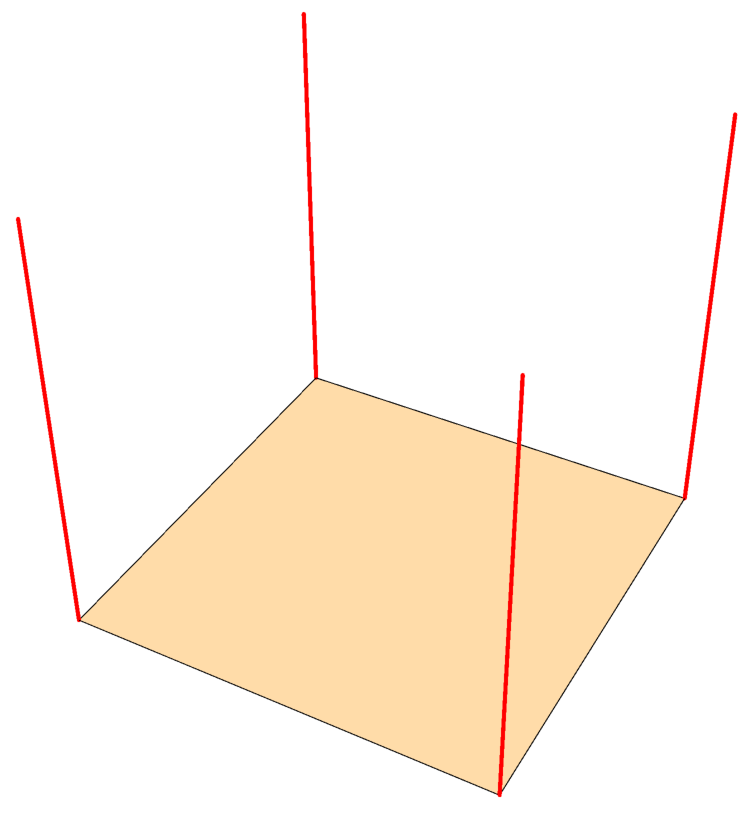
\includegraphics[ width = 0.8in ]{../graphics/defects/array11_pbc/nullspace.pdf} &
      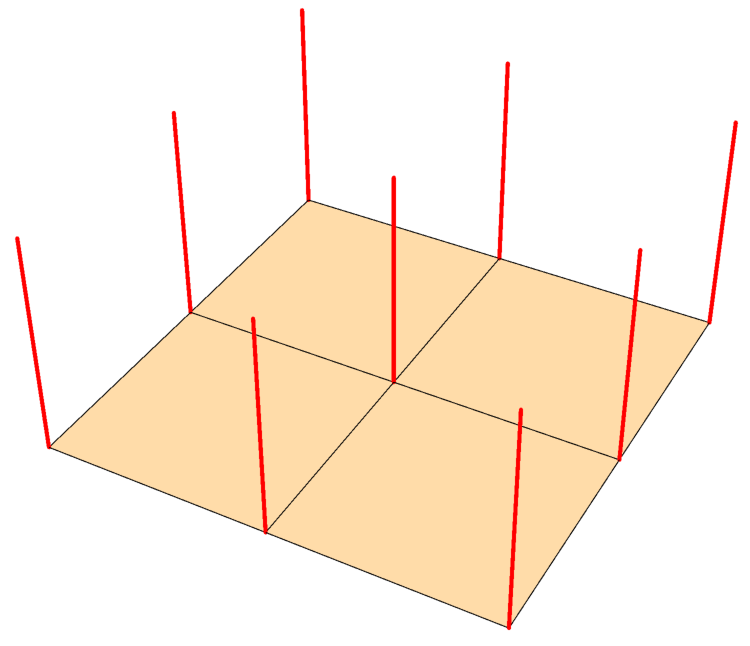
\includegraphics[ width = 1in ]{../graphics/defects/array22_pbc/nullspace.pdf} \\
      %
      
\includegraphics[ width = 0.75in ]{../graphics/defects/array11_pbc/verify} &
      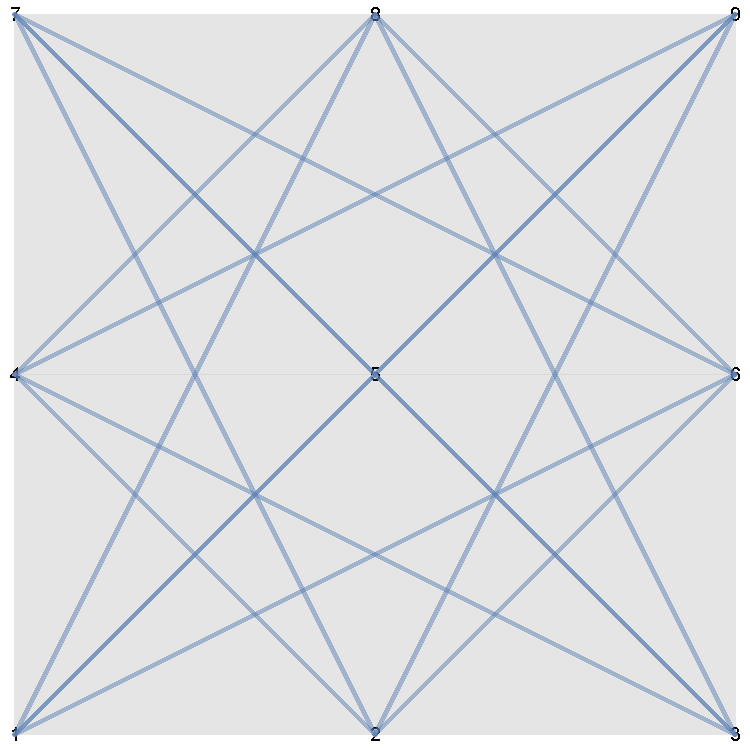
\includegraphics[ width = 0.75in ]{../graphics/defects/array22_pbc/verify}
      %
      %
    \end{tabular}
  \end{center}
  %\label{default}
  %\caption{default}
\end{table}%
  %
\end{frame}

\begin{frame}      %  %  %   FRAME   %  %  %
\frametitle{Rank Defect 2: Squares}
  %
\begin{table}[htdp]
  \begin{center}
    \begin{tabular}{ccc}
      %
      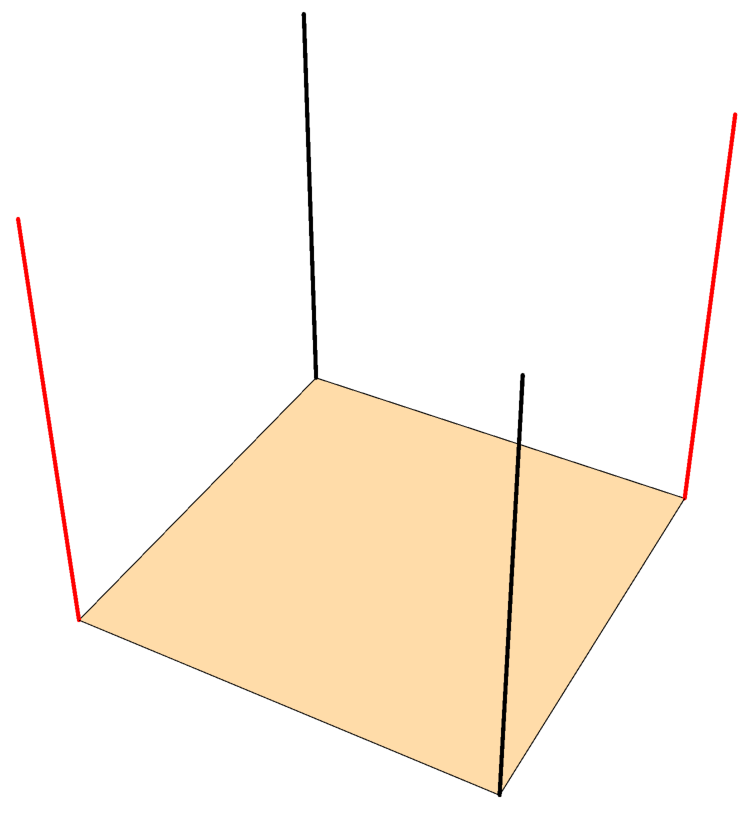
\includegraphics[ width = 0.8in ]{../graphics/defects/array11/nullspace.pdf} &
      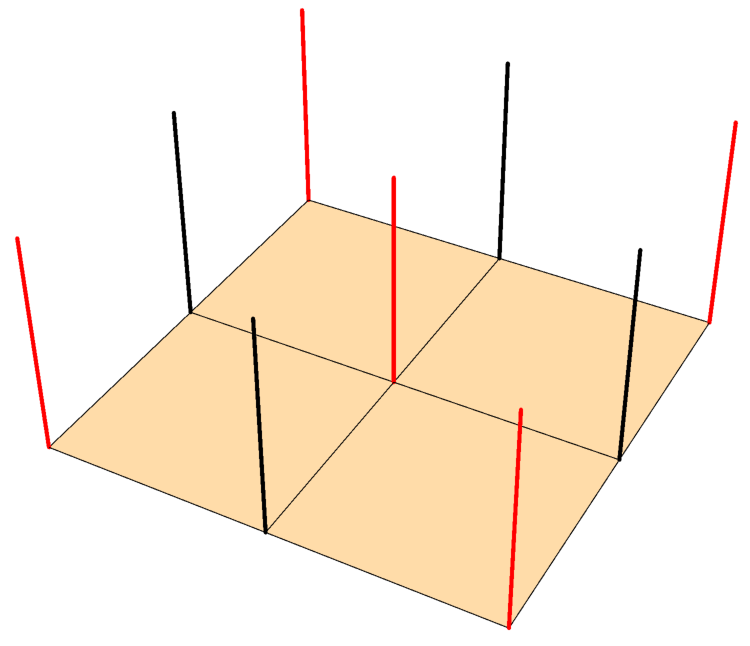
\includegraphics[ width = 0.8in ]{../graphics/defects/array22/nullspace.pdf} &
      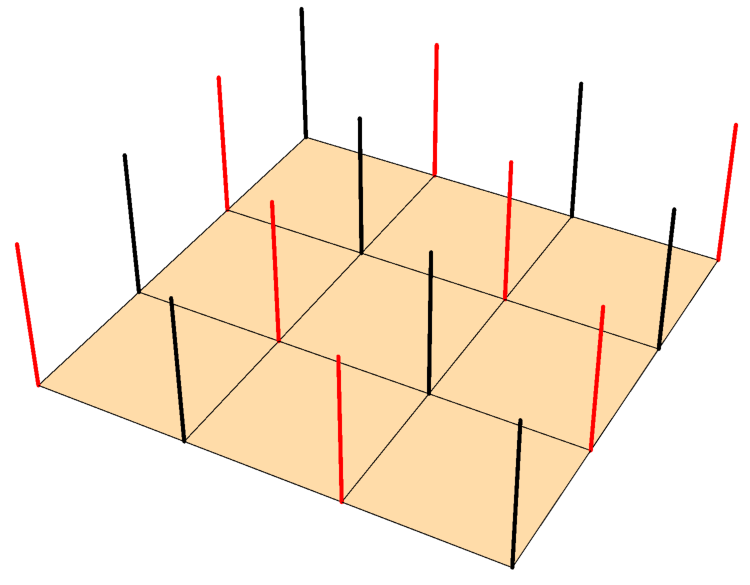
\includegraphics[ width = 1.0in ]{../graphics/defects/array33/nullspace.pdf} \\
      %
      
\includegraphics[ width = 0.75in ]{../graphics/defects/array11/verify} &
      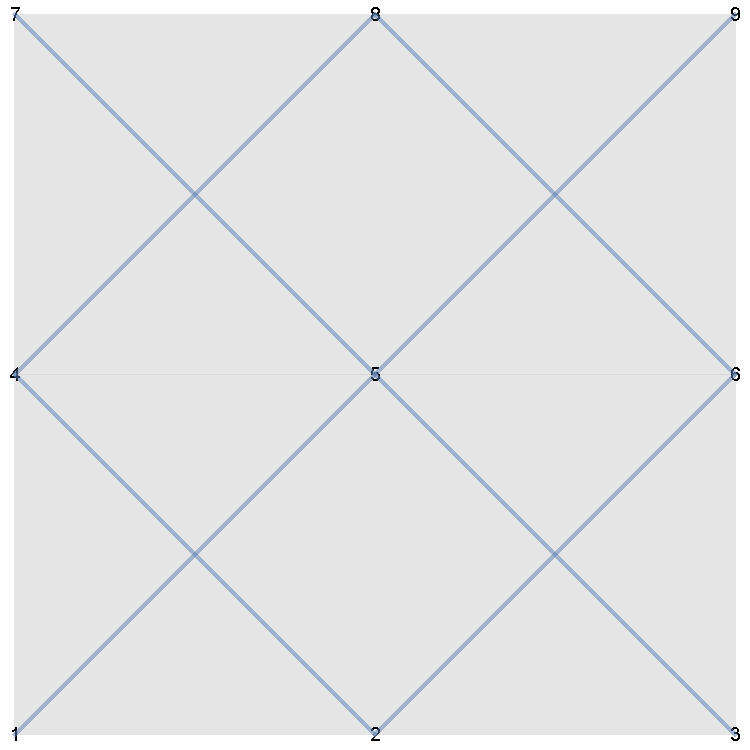
\includegraphics[ width = 0.75in ]{../graphics/defects/array22/verify} &
      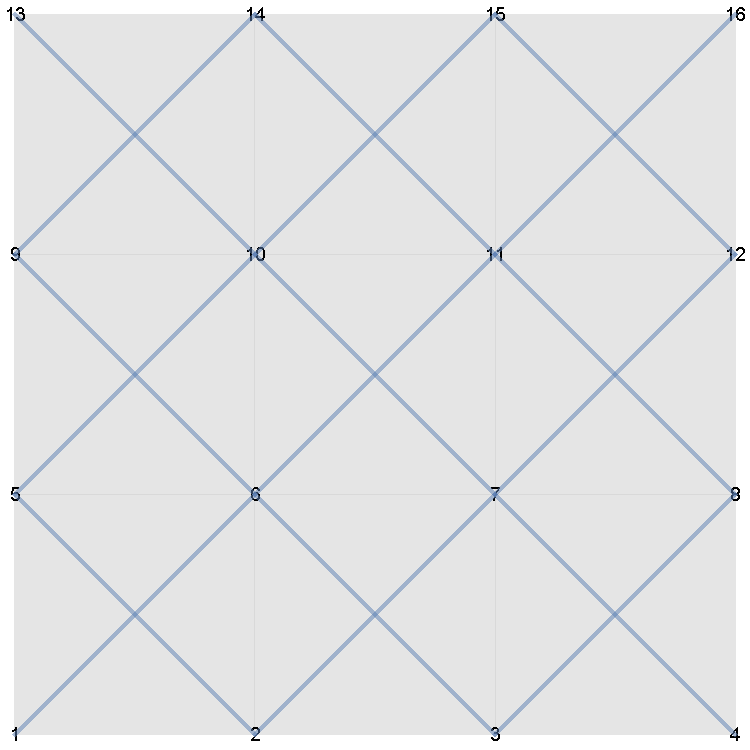
\includegraphics[ width = 0.75in ]{../graphics/defects/array33/verify}
      %
      %
    \end{tabular}
  \end{center}
  %\label{default}
  %\caption{default}
\end{table}%
  %
\end{frame}

\begin{frame}      %  %  %   FRAME   %  %  %
\frametitle{Rank Defect 2: Irregulars}
  %
\begin{table}[htdp]
  \begin{center}
    \begin{tabular}{ccc}
      %
      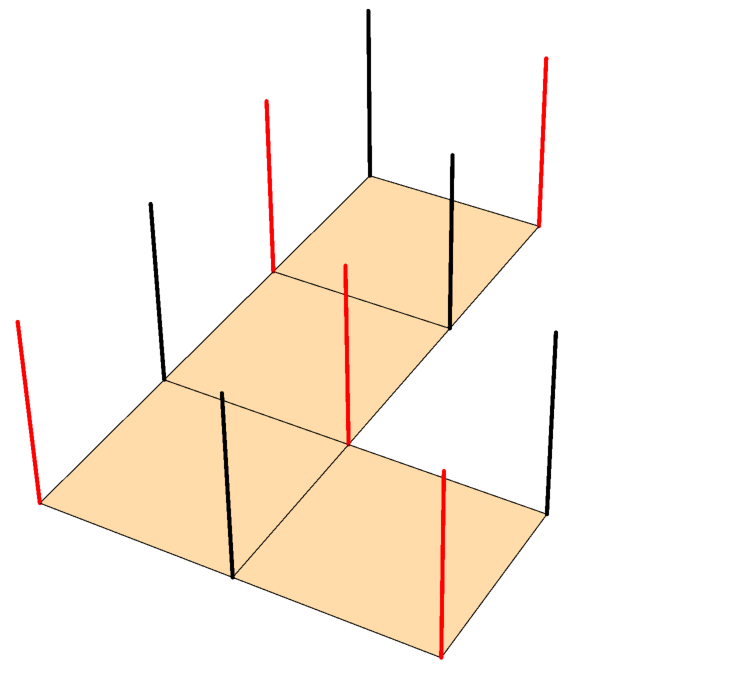
\includegraphics[ width = 0.8in ]{../graphics/defects/L/nullspace.pdf} &
      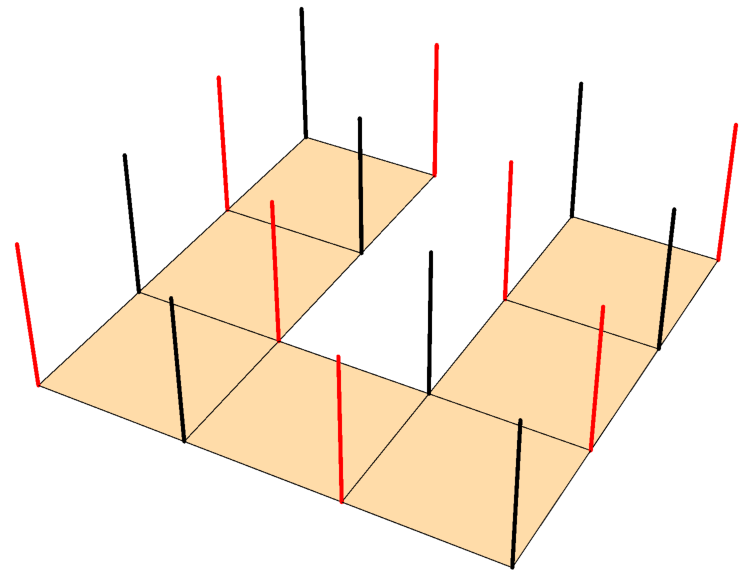
\includegraphics[ width = 0.8in ]{../graphics/defects/U/nullspace.pdf} &
      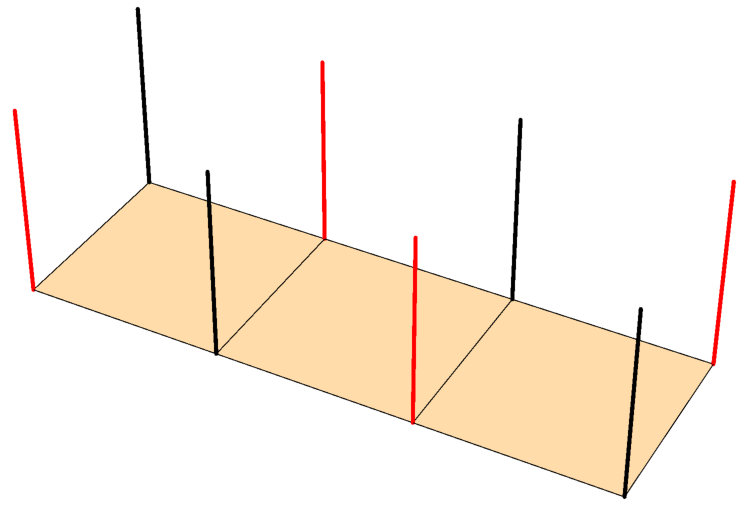
\includegraphics[ width = 1.0in ]{../graphics/defects/array13/nullspace.pdf} \\
      %
      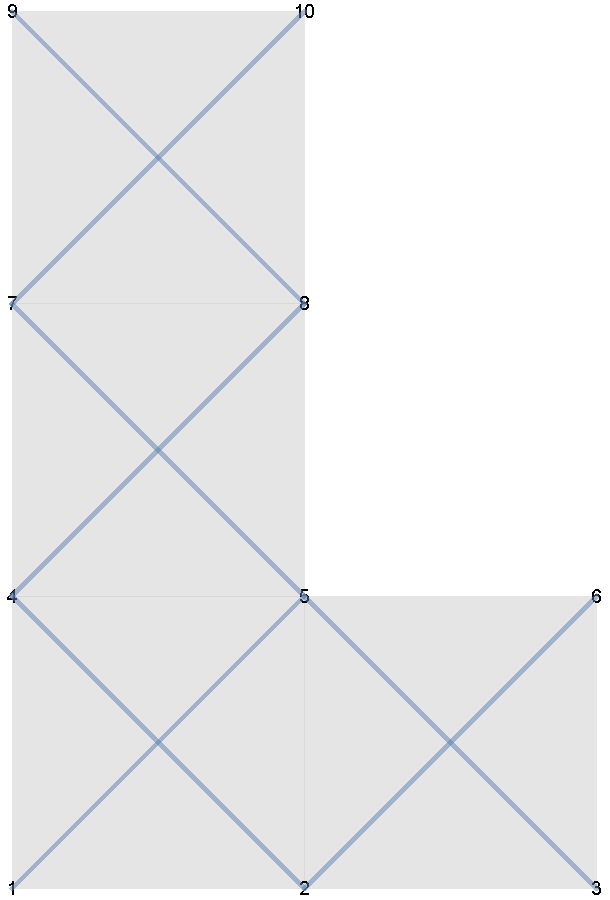
\includegraphics[ width = 0.75in ]{../graphics/defects/L/verify} &
      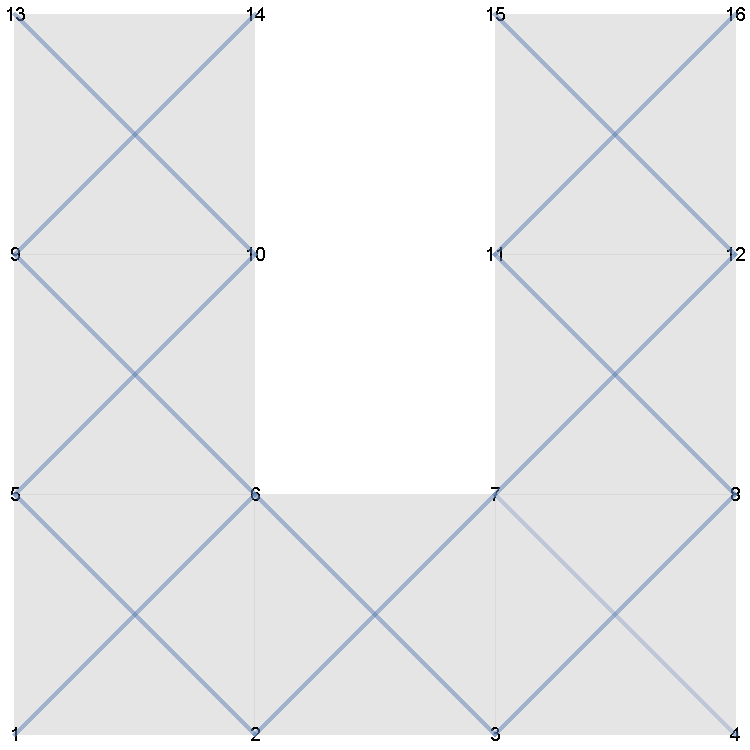
\includegraphics[ width = 1.125in ]{../graphics/defects/U/verify} &
      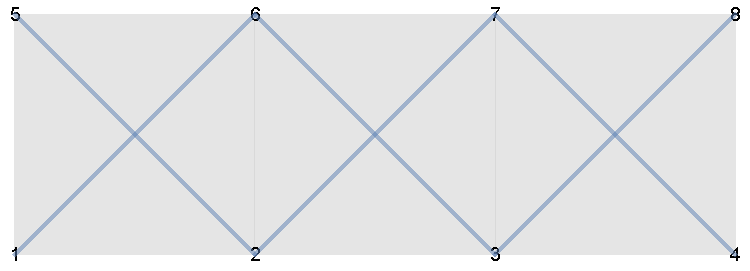
\includegraphics[ width = 1.125in ]{../graphics/defects/array13/verify}
      %
      %
    \end{tabular}
  \end{center}
  %\label{default}
  %\caption{default}
\end{table}%
  %
\end{frame}

\begin{frame}      %  %  %   FRAME   %  %  %
\frametitle{Rank Defect 3}
  %
  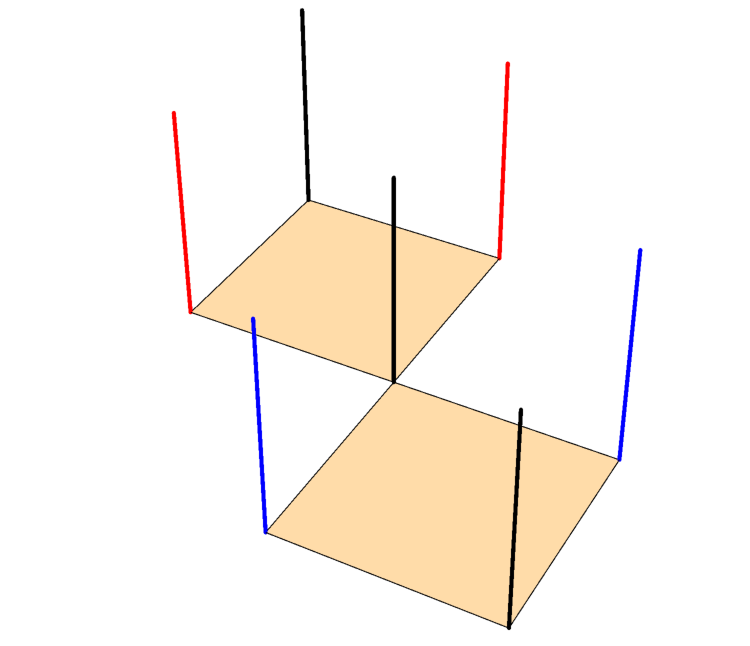
\includegraphics[ width = 2in ]{../graphics/defects/stairs2/nullspace.pdf} \qquad
  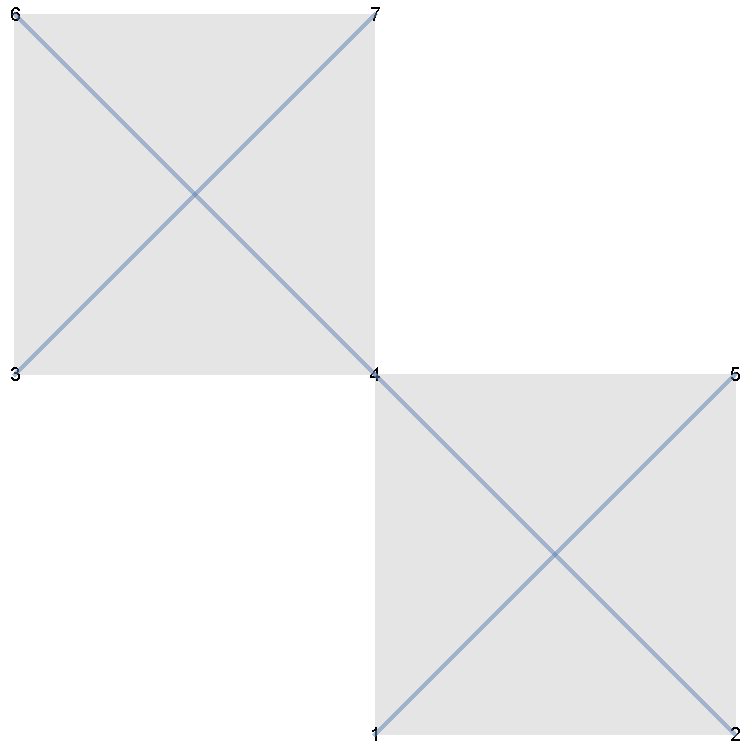
\includegraphics[ width = 1.5in ]{../graphics/defects/stairs2/verify.pdf}
  %
\end{frame}

\begin{frame}      %  %  %   FRAME   %  %  %
\frametitle{Rank Defect 4}
  %
\begin{table}[htdp]
  \begin{center}
    \begin{tabular}{cc}
      %
      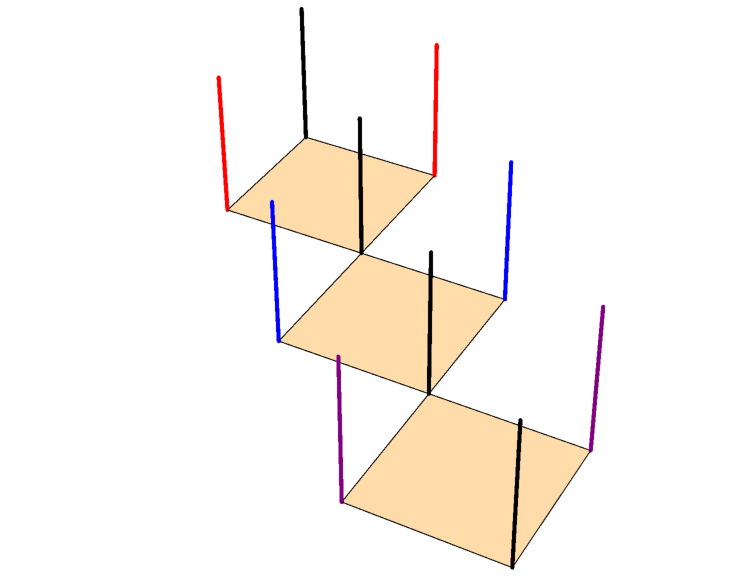
\includegraphics[ width = 1.35in ]{../graphics/defects/stairs3/nullspace.pdf} &
      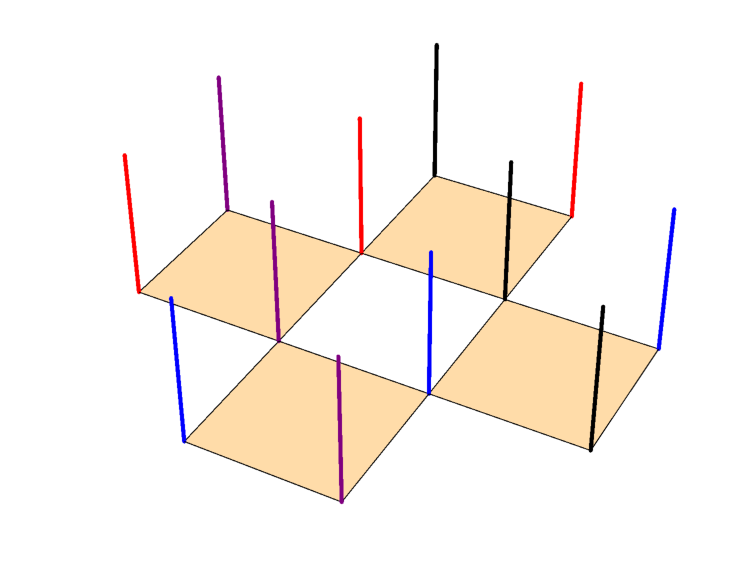
\includegraphics[ width = 1.5in ]{../graphics/defects/checkerboard_ring/nullspace.pdf} \\
      %
      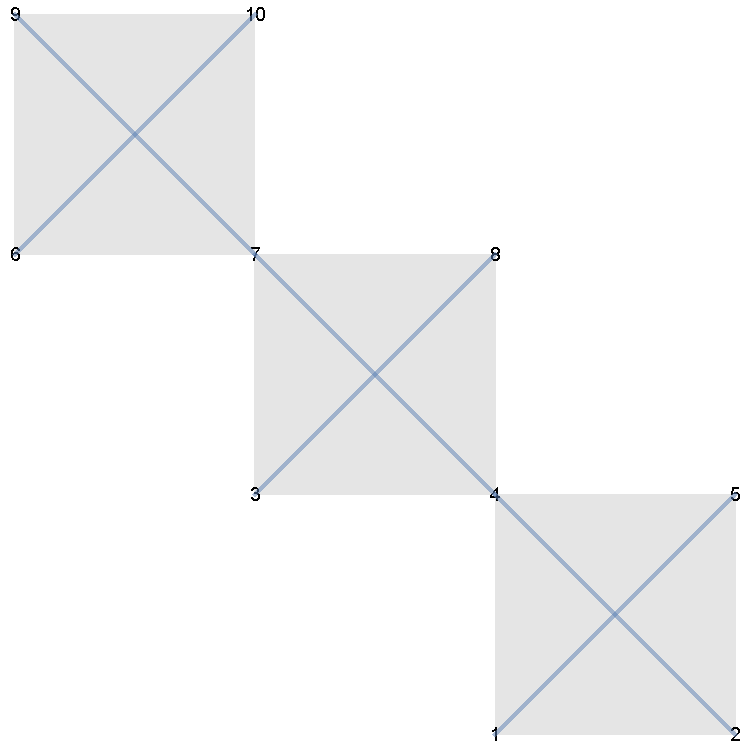
\includegraphics[ width = 1.125in ]{../graphics/defects/stairs3/verify} &
      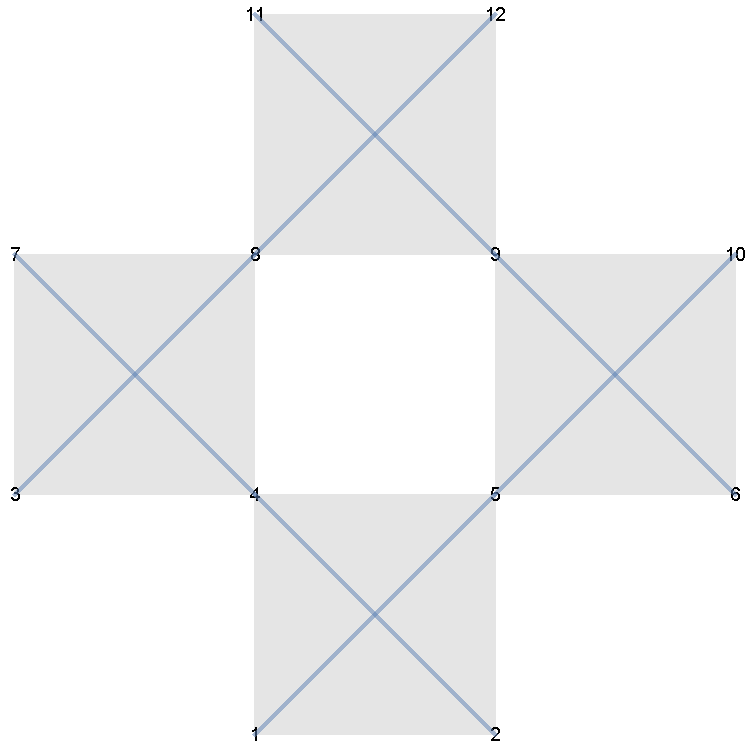
\includegraphics[ width = 1.125in ]{../graphics/defects/checkerboard_ring/verify}
      %
      %
    \end{tabular}
  \end{center}
  %\label{default}
  %\caption{default}
\end{table}%
  %
\end{frame}

\begin{frame}      %  %  %   FRAME   %  %  %
\frametitle{Rank Defect 6}
  %
  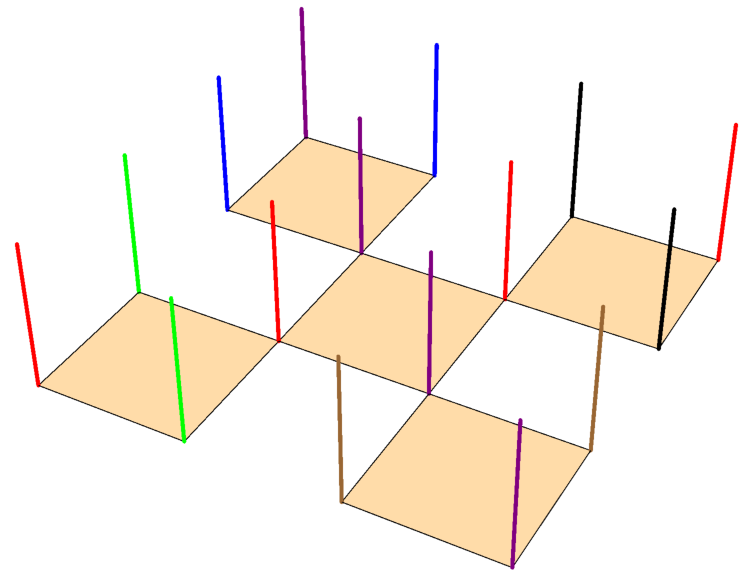
\includegraphics[ width = 2in ]{../graphics/defects/checkerboard_ring_complement/nullspace.pdf} \qquad
  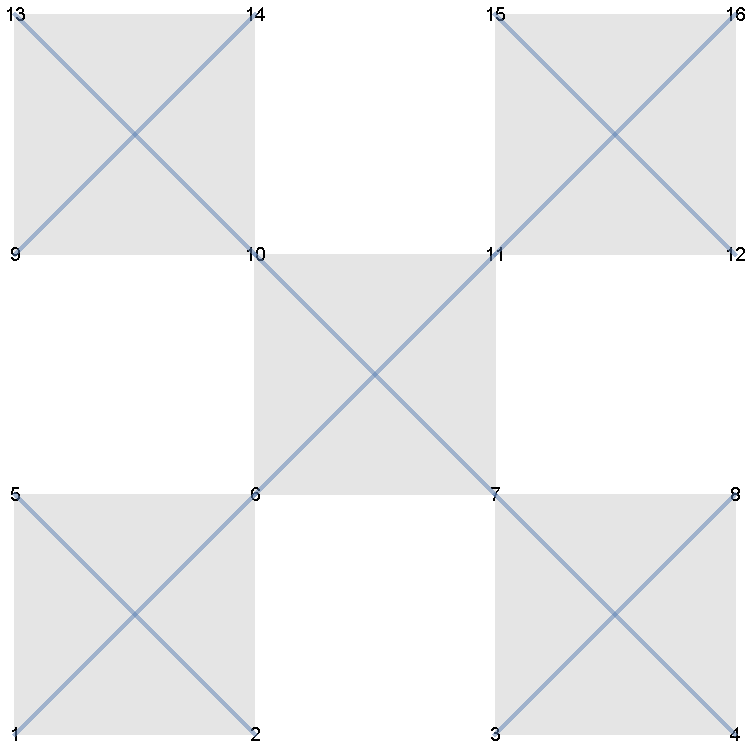
\includegraphics[ width = 1.5in ]{../graphics/defects/checkerboard_ring_complement/verify.pdf}
  %
\end{frame}

%  %  %  %  %  %  %  %  %  %  %  %  %  %  %  %  %  %  %  %  %  %  %  %  %  %  %  %  %  %  %  %  %  %  %  %  %  %  %  %  %  %  %  %  %  %  %
\section{Closing}

\begin{frame}      %  %  %   FRAME   %  %  %
\frametitle{Summary}
  %
  \begin{enumerate}
    \item \mg{Measure vector field $\bf{F}$}
    \item Construct $\A{} = \csvdblockb{*}$
    \item Construct null space vectors
    \item Create $\A{} = \csvdblockbc{*}$
    \item \mg{Solve for potential s.t. $\bf{F} = \nabla \phi$}
  \end{enumerate}
  %
\end{frame}


\begin{frame}      %  %  %   FRAME   %  %  %
\frametitle{Acknowledgements}
%
\begin{table}[htdp]
  %\caption{default}
  \begin{center}
    \begin{tabular}{cl}
      %
      
\includegraphics[ width = 2cm ]{../graphics/logos/UNM} &
      \raisebox{1.1\height}{\tiny{Mathematics and Statistics}} \\[20pt]
      %
      \includegraphics[ width = 2cm ]{../graphics/logos/HPCMP} &
      \raisebox{2.75\height}{\tiny{High Performance Computing Modernization Program  (HPCMP)}} \\[-18pt]
      %
      & \tiny{Productivity Enhancement, Technology Transfer and Training (PETTT)}
      %
    \end{tabular}
  \end{center}
  %\label{default}
\end{table}%
%
\end{frame}

\tpage

\end{document}


%\tiny
%\scriptsize
%\footnotesize
%\small
%\normalsize
%\large
%\Large
%\LARGE
%\huge
%\Huge

%\, thin space (normally 1/6 of a quad);
%\> medium space (normally 2/9 of a quad);
%\; thick space (normally 5/18 of a quad);
%\! negative thin space (normally 1/6 of a quad).
